\documentclass{article}
\usepackage[final]{neurips_2023}
\usepackage{amsfonts}
\usepackage[mathscr]{euscript}
\usepackage[numbers]{natbib} % has a nice set of citation styles and commands
\usepackage{mathtools} % amsmath with fixes and additions
\usepackage{bbm}
% \usepackage{siunitx} % for proper typesetting of numbers and units
\usepackage{booktabs} % commands to create good-looking tables
\usepackage{tikz} % nice language for creating drawings and diagrams
% \usepackage{algorithm2e}
\usepackage{boxedminipage}
\usepackage{alltt}
\usepackage{bm}
\usepackage{hyperref}
\usepackage{authblk}
\usepackage{multirow}
\usepackage{makecell}
\usepackage{algorithm}
\usepackage{algorithmic}

\title{Multi-Task Offline Reinforcement Learning with Heuristic Conservative Soft Actor-Critic\\
\vspace{0.5em} \normalsize Project of AI3601 Reinforcement Learning, 2024 Spring, SJTU}
\author{Jiazi Bu$^{\ast}$, Kailing Wang$^{\ast}$, Xiangyuan Xue$^{\ast\dagger}$}
\affil[]{School of Electronic Information and Electrical Engineering\\
\footnotesize $^\ast$Equal Contribution \quad $^\dagger$Project Leader}

\begin{document}

\maketitle

\begin{abstract}
In this project, we propose a novel method named heuristic conservative soft actor-critic (HCSAC) based on conservative Q-learning (CQL) and soft actor-critic (SAC) to solve the offline multi-task reinforcement learning problem. We employ task embedding to allow the agent to learn shared representations across multiple tasks. We also follow conservative data sharing (CDS) to utilize heuristic relabeling to augment the offline dataset, so that the agent can benefit from the shared transitions while avoiding performance degradation. We conduct a series of experiments on the MuJoCo benchmark to verify the effectiveness of our method. The results show that our proposed methods in general bring superior performance and improve the robustness of the agent.
\end{abstract}

\section{Introduction}
\label{sec:introduction}

Reinforcement learning (RL) describes the sequential decision-making process where an agent interacts with the environment to maximize the cumulative reward signal \cite{sutton1999reinforcement}. With the development of deep learning, deep reinforcement learning (DRL) has emerged as a powerful paradigm that combines deep neural networks with traditional reinforcement learning algorithms, making it possible to learn complex behavior representations from high-dimensional sensory inputs \cite{li2017deep}. Such paradigm empowers the agent to learn effective behavior policies in various real-world scenarios such as robotics control \cite{kober2013reinforcement}, game playing \cite{silver2018general}, and autonomous driving \cite{kiran2021deep}.

In the traditonal setting, the agent learns in an online manner, which requires the agent to frequently interact with the environment to gather samples. However, such interaction can be extremely expensive in some real-world applications. On one hand, collecting real-world samples can hardly be parallelized, which makes the process remarkably slow. On the other hand, the agent may suffer from catastrophic failures during the learning process, which may not be affordable in safety-critical applications. To address these issues, researchers have proposed an alternative offline manner, where the agent learns from a fixed dataset without interacting with the environment \cite{levine2020offline} as shown in Figure \ref{fig:offline_rl}. Admittedly, the offline reinforcement learning paradigm is attractive, but it also faces several challenges. The bootstrap method unavoidably introduces distribution shifts, which makes the traditional algorithms fail to learn a satisfactory policy. Researchers have proposed various methods to tackle this problem, such as implicit Q-learning \cite{kostrikov2021offline}, conservative Q-learning \cite{kumar2020conservative}, and TD3-BC \cite{fujimoto2021minimalist}. The core idea of these methods is to suppress the overestimation of the Q-value function, which is widely recognized as the main reason for the failure of offline reinforcement learning.

\begin{figure}[ht]
    \centering
    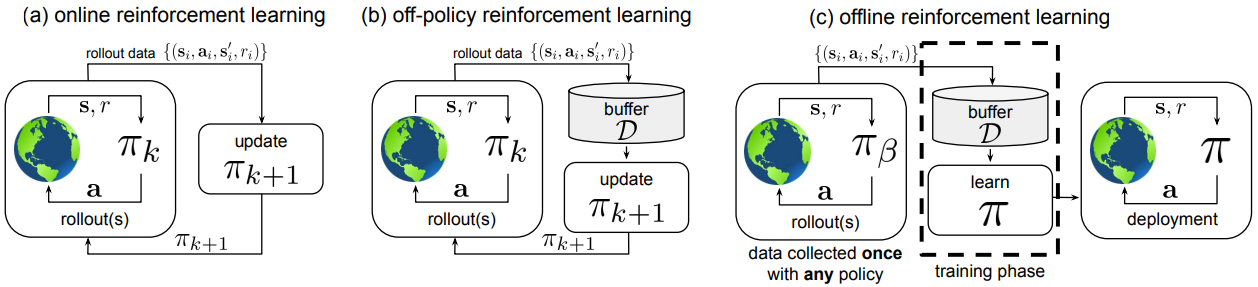
\includegraphics[width=0.9\textwidth]{figure/offline_rl.png}
    \caption{An illustration of online reinforcement learning, off-policy reinforcement learning, and offline reinforcement learning. Offline reinforcement learning follows an open-loop control paradigm, where the agent learns from a fixed dataset without interacting with the environment.}
    \label{fig:offline_rl}
\end{figure}

When it comes to scaling up the reinforcement learning algorithms, researchers find that learning multiple tasks simultaneously can effectively improve the sample efficiency and generalization ability of the agent as shown in Figure \ref{fig:multi_task}. Multi-task reinforcement learning (MTRL) thus becomes a popular research direction in recent years \cite{vithayathil2020survey}. Researchers have proposed various methods for the multi-task setting, including shared representation learning \cite{borsa2016learning}, knowledge transfer and distillation \cite{xu2020knowledge}, and progressive neural networks \cite{rusu2016progressive}. However, most of these methods are designed for the online setting, so they will suffer from the same issues when applied to the offline setting. Some novel methods have been proposed to combine the offline and multi-task learning paradigms, such as conservative data sharing \cite{yu2021conservative} and scaled Q-learning \cite{kumar2022offline}, but how to achieve reliable offline multi-task reinforcement learning still remains an open problem till today.

\begin{figure}[ht]
    \centering
    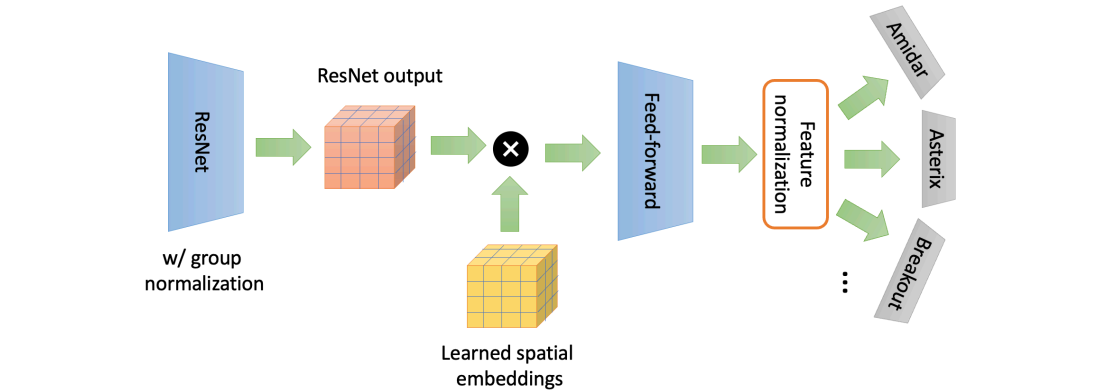
\includegraphics[width=0.9\textwidth]{figure/multi_task.png}
    \caption{An example of multi-task reinforcement learning. Multiple policy heads share the same backbone as the feature extractor to learn useful shared representations, so that the agent can benefit from the extensive experience and knowledge transfer across multiple tasks.}
    \label{fig:multi_task}
\end{figure}

In this project, we aim to explore the offline multi-task reinforcement learning paradigm. Our study pivots around improving the sample efficiency and generalization ability of the agent by fully exploiting the potential of multi-task learning. We propose a novel algorithm framework named heuristic conservative soft actor-critic (HCSAC) to solve the offline multi-task reinforcement learning problem. The framework is built upon the conservative Q-learning \cite{kumar2020conservative} and soft actor-critic \cite{haarnoja2018soft} algorithms to suppress distribution shifts in the offline setting. We also introduce task embeddings to allow the agent to learn shared representations across multiple tasks. In addition, we follow conservative data sharing \cite{yu2021conservative} and propose a heuristic strategy to relabel the dataset, so that the agent can benefit from the augmented transitions while avoiding performance degradation. We conduct a series of experiments on the MuJoCo benchmark \cite{todorov2012mujoco} to evaluate the performance of our method. Through these efforts, we expect to provide some insights into the characteristics and efficacies of the proposed method, and to demonstrate the potential of offline multi-task reinforcement learning in real-world applications.
\section{Method}
\label{sec:method}

\subsection{Preliminaries}

The goal of reinforcement learning is to learn a policy that maximizes the expected cumulative discounted reward in a Markov decision process (MDP) \cite{sutton1999reinforcement} defined by the tuple $(\mathcal{S}, \mathcal{A}, P, R, \gamma)$, where $\mathcal{S}$ is the state space, $\mathcal{A}$ is the action space, $P(s'|s, a)$ is the transition probability, $R(s, a)$ is the reward function, and $\gamma \in (0, 1)$ is the discount factor. The agent interacts with the environment by following a policy $\pi(a|s)$, which maps states to actions. The state value function $V^{\pi}(s)$ and the action-value function $Q^{\pi}(s, a)$ are defined as the expected cumulative discounted reward under policy $\pi$ starting from state $s$ and taking action $a$. The optimal value functions $V^*(s)$ and $Q^*(s, a)$ are defined as the maximum value functions over all policies, which satisfy the Bellman equation
\begin{equation}
    \begin{aligned}
        V^*(s) &= \max_{\pi} \mathbb{E}_{a \sim \pi(\cdot|s)} \left[ Q^{\pi}(s, a) \right] \\
        Q^*(s, a) &= R(s, a) + \gamma \mathbb{E}_{s' \sim P(\cdot|s, a)} \left[ \max_{a'} Q^*(s', a') \right]
    \end{aligned}
\end{equation}
In the offline setting, the environment is not accessible when training, so the agent can only learn from a fixed dataset $\mathcal{D} = \{(s_i, a_i, r_i, s'_i)\}_{i=1}^N$ collected by a behavior policy $\pi_{\beta}(a|s)$, where $s_i$ is the state, $a_i$ is the action, $r_i$ is the reward, $s'_i$ is the next state, and $N$ is the number of transitions. In the multi-task setting, the dataset $\mathcal{D}=\cup_{i=1}^M \mathcal{D}_i$ consists of transitions from multiple tasks, where $\mathcal{D}_i$ is the dataset of task $i$ and $M$ is the number of tasks. The goal is to learn a policy that maximizes the expected cumulative discounted reward across all the tasks.

\subsection{Soft Actor-Critic}

Soft actor-critic (SAC) is an actor-critic algorithm that maximizes the entropy-regularized expected cumulative discounted reward \cite{haarnoja2018soft}. Different from the traditional actor-critic algorithms such as trust region policy optimization (TRPO) \cite{schulman2015trust} and proximal policy optimization (PPO) \cite{schulman2017proximal}, SAC follows an off-policy learning paradigm, which significantly improves the sample efficiency and can be better applied to the offline setting. Besides the cumulative reward, SAC also tries to maximize the entropy of the policy, which encourages exploration and prevents premature convergence to suboptimal policies. The objective function of SAC can be specified as
\begin{equation}
    J(\pi) = \sum \nolimits_{t=0}^{\infty} \mathbb{E}_{(s_t, a_t) \sim \rho_{\pi}} \left[ R(s_t, a_t) + \alpha \mathcal{H}(\pi(\cdot|s_t)) \right]
\end{equation}
where $\rho_{\pi}$ is the state-action visitation distribution induced by the policy $\pi$, $\mathcal{H}(\pi(\cdot|s_t))$ is the entropy of the policy, and $\alpha$ is the temperature parameter that determines the relative importance of the entropy term. Then the policy evaluation step should be modified to match the entropy-regularized objective. The soft Q-value can be computed by iteratively applying a modified Bellman operator
\begin{equation}
    \mathcal{T}^{\pi}Q(s, a) = R(s, a) + \gamma \mathbb{E}_{s' \sim P(\cdot|s, a)} \left[ \mathbb{E}_{a' \sim \pi(\cdot|s')} \left[ Q(s', a') - \alpha \log \pi(a'|s') \right] \right]
\end{equation}
Theoretical analysis shows that the soft Q-value will finally converge with enough iterations. At the same time, the policy improvement step should also be modified. SAC assumes that the policy distribution is proportional to the exponential of the soft Q-value, so the policy can be updated by minimizing the Kulback-Leibler (KL) divergence between the current policy and the normalized exponential of the soft Q-value, which can be formulated as
\begin{equation}
    \pi'(\cdot|s) = \arg \min_{\mu} D_{\text{KL}} \left( \mu(\cdot|s) \left\| \frac{\exp(Q^{\pi}(s, \cdot))}{Z^{\pi}(s)} \right. \right)
\end{equation}
where $Z^{\pi}(s)$ is the partition function that normalizes the exponential of the soft Q-value. Theoretical analysis shows that the policy is guaranteed to improve, so it will converge to the optimal policy.

In the actual implementation, several tricks are introduced to realize the expected algorithm. Firstly, SAC uses a Gaussian policy parameterized by a mean and a standard deviation, so the reparameterization trick is required to back propagate the gradient correctly. Secondly, SAC uses two Q-networks to estimate the soft Q-value and takes the minimum of the two results to avoid the overestimation of the Q-value. SAC also introduces two target Q-networks as in deep deterministic policy gradient (DDPG) \cite{lillicrap2015continuous} to update the Q-networks softly and stabilize the training process. Finally, we introduce automating entropy adjustment for maximum entropy \cite{haarnoja2018application} to adaptively choose the temperature parameter $\alpha$ during training. To be specific, it converts the entropy regularization term into a constraint and tries to solve the following constrained optimization problem
\begin{equation}
    \begin{aligned}
        \max_{\pi} & \sum \nolimits_{t=0}^{\infty} \mathbb{E}_{(s_t, a_t) \sim \rho_{\pi}} \left[ R(s_t, a_t) \right] \\
        \text{s.t. } & \mathbb{E}_{(s_t, a_t) \sim \rho_{\pi}} \left[ -\log \pi(a_t|s_t) \right] \geq \mathcal{H}_0, \forall t
    \end{aligned}
\end{equation}
where $\mathcal{H}$ is the target entropy. This constrained optimization problem can be converted into its dual form and solved by the Lagrange multiplier method. The result can be formulated as
\begin{equation}
    \alpha_t^* = \arg \min_{a_t} \mathbb{E}_{a_ t\sim \pi(\cdot|s_t)} \left[ - \alpha_t \log \pi(a_t|s_t) - \alpha_t \mathcal{H}_0 \right]
\end{equation}
where $\bar{\mathcal{H}}$ is a predefined minimum policy entropy threshold, which is empirically set to the negative of the action space dimension. Now the temperature parameter $\alpha$ can be automatically adjusted during the training process by gradient descent method. This trick is proved to be quite effective in practice and has been widely used in the SAC algorithm.

\subsection{Conservative Q-Learning}

Although researchers have proposed many methods for offline reinforcement learning, conservative Q-learning (CQL) \cite{kumar2020conservative} is still the most stable and effective method in practice. The key idea of CQL is to discourage the out-of-distribution Q-values while encouraging the Q-values in the dataset, so that the overestimation of the Q-values can be suppressed to some extent. The original form of CQL can be formulated as a family of optimization problems
\begin{equation}
    \begin{aligned}
        \min_Q \max_{\mu} &\ \alpha \left( \mathbb{E}_{s \sim \mathcal{D}, a \sim \mu(\cdot|s)} \left[ Q(s, a) \right] - \mathbb{E}_{s \sim \mathcal{D}, a \sim \pi_{\beta}(\cdot|s)} \left[ Q(s, a) \right] \right) \\
        &+ \frac{1}{2} \mathbb{E}_{(s,a,s') \sim \mathcal{D}} \left[ \left( Q(s, a) - \mathcal{B}^{\pi_k} Q^k(s, a) \right)^2 \right] + \mathcal{R}(\mu)
    \end{aligned}
\end{equation}
where $\alpha$ is the temperature parameter that determines the relative importance of the conservative term, $\mathcal{B}^{\pi_k}$ is the Bellman operator under the behavior policy $\pi_k$, and $\mathcal{R}(\mu)$ is a general regularizer. If we choose $\mathcal{R}(\mu)$ to be the KL divergence between the current policy and the uniform distribution, the optimization problem can be rearranged into the following form
\begin{equation}
    \begin{aligned}
        \min_Q &\ \alpha \mathbb{E}_{s \sim \mathcal{D}} \left[ \log \sum \nolimits_a \exp(Q(s, a)) - \mathbb{E}_{a \sim \pi_{\beta}(\cdot|s)} \left[ Q(s, a) \right] \right] \\
        &+ \frac{1}{2} \mathbb{E}_{(s,a,s') \sim \mathcal{D}} \left[ \left( Q(s, a) - \mathcal{B}^{\pi_k} Q^k(s, a) \right)^2 \right]
    \end{aligned}
\end{equation}
In continuous action spaces, the log-sum-exp operation should be approximated by importance sampling, where we can rewrite the term as
\begin{equation}
    \begin{aligned}
        \log \sum \nolimits_a \exp(Q(s, a)) &= \log \left( \frac{1}{2} \sum \nolimits_a \exp(Q(s, a)) + \frac{1}{2} \sum \nolimits_a \exp(Q(s, a)) \right) \\
        &= \log \left( \frac{1}{2} \mathbb{E}_{a\sim U(\mathcal{A})} \left[ \frac{\exp(Q(s, a))}{U(a)} \right] + \frac{1}{2} \mathbb{E}_{a\sim \pi(\cdot|s)} \left[ \frac{\exp(Q(s, a))}{\pi(a|s)} \right] \right)
    \end{aligned}
\end{equation}
where $U(\mathcal{A})$ is the uniform distribution over the action space. Then we can sample $N$ actions each from the uniform distribution and the policy distribution to effectively estimate this term. Note that CQL only makes some modifications to the objective function of the Q-network, so it can be easily combined with other actor-critic algorithms. In practice, CQL is usually combined with SAC to solve the offline reinforcement learning problems with continuous action spaces.

\subsection{Task Embedding}

Since we expect the agent to learn multiple tasks simultaneously, we need a machanism to explicitly inform the agent of which task it is currently facing. The simplest way is to separately train a policy for each task, but this method is not efficient enough and cannot fully exploit the shared representations among tasks. Scaled Q-learning \cite{kumar2022offline} uses multiple policy heads for each task which share the same backbone as the feature extractor, so that the agent can benefit from the shared feature representations across tasks. Conservative data sharing \cite{yu2021conservative} appends a one-hot vector to the state space to indicate the task, so that the agent can distinguish the tasks and learn specific policies.

Inspired by the embeddings used in transformers, we propose a similar method to specify the task information. As shown in Figure \ref{fig:task_embedding}, we assign a unique identity $k$ to each task. The identity will be fed into an embedding layer to generate the task embedding $e$, which will be added onto the state $s$ as the task-aware state $z$. The task-aware state $z$ will be fed together with the action $a$ into the critic network to output the estimated Q-value $\hat{q}$. It will also be fed alone into the actor network to output the predicted action $\hat{a}$. Note that the task embedding $e$ can be learned during the training process, which ensures that the performance of the agent will not degrade in the multi-task setting.

\begin{figure}[ht]
    \centering
    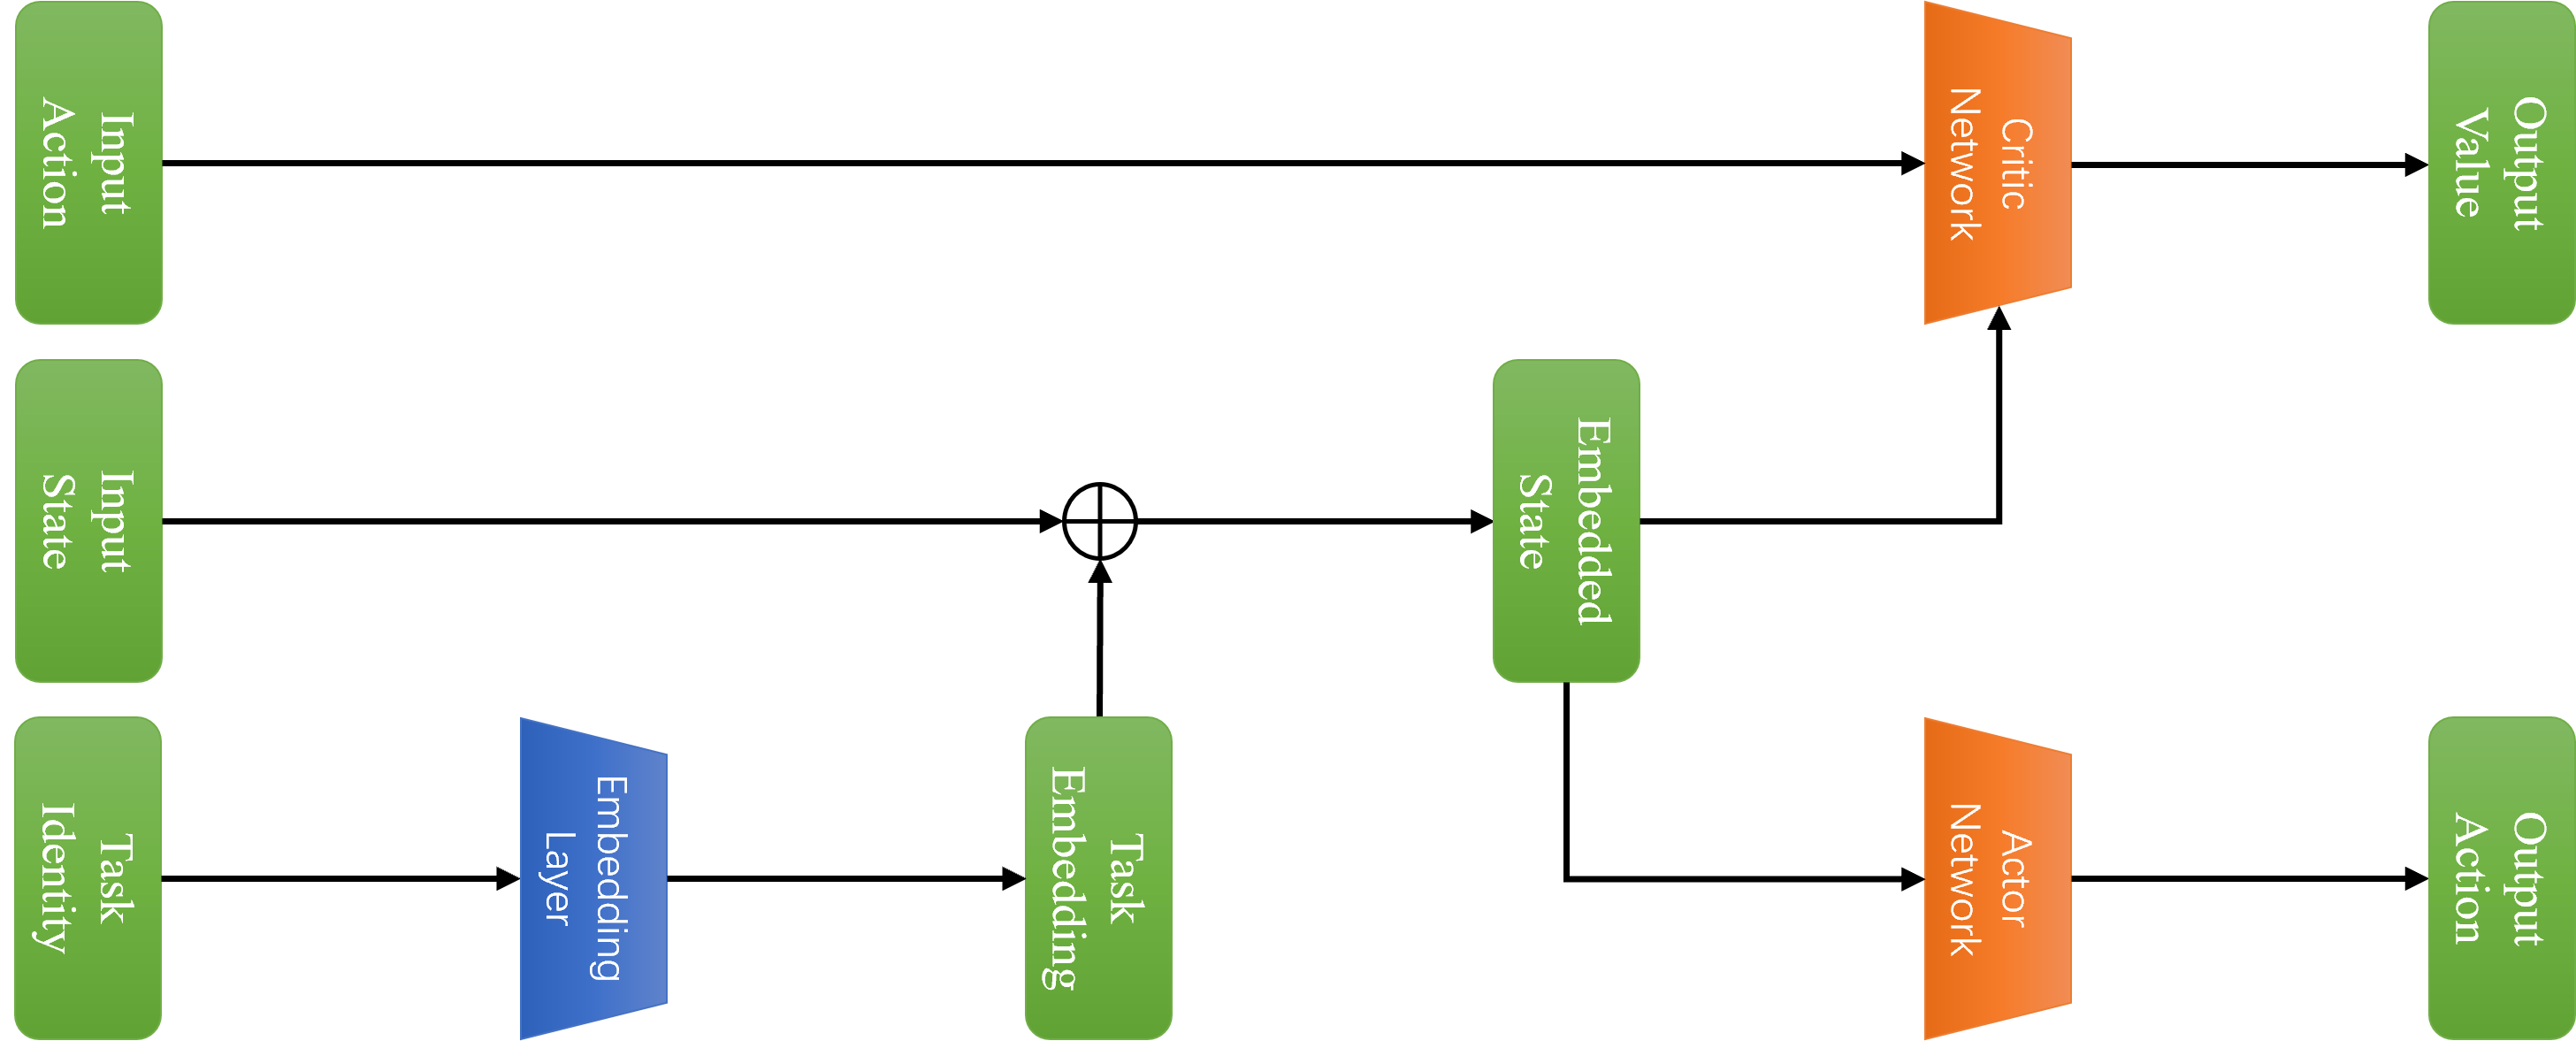
\includegraphics[width=0.8\textwidth]{figure/task_embedding.png}
    \caption{An illustration of the task embedding. The task identity $k$ is fed into an embedding layer to generate the task embedding $e$, which will be added onto the state $s$ as the task-aware state $z$. The task-aware state $z$ will be fed together with the action $a$ into the critic network to output the estimated Q-value $\hat{q}$. It will also be fed alone into the actor network to output the predicted action $\hat{a}$.}
    \label{fig:task_embedding}
\end{figure}

\subsection{Heuristic Relabeling}

Previous works \cite{yu2021conservative} have verified that one of the main reason for the failure in the multi-task setting is distribution shifts. If the agent utilizes the transitions from all the tasks without making any distinction, those out-of-distribution transitions will significantly hinder the learning process. Inspired by the idea of conservative data sharing \cite{yu2021conservative}, one feasible solution is to share the transitions conservatively. Luckily, conservative Q-learning has already provided the conservative Q-values as an indicator to measure the distribution shifts, so we define the relabeling threshold $\tau(\mathcal{D}_i)$ as
\begin{equation}
    \tau(\mathcal{D}_i) = \left\{ Q_i(s, a) | (s, a) \in \mathcal{D}_i \right\}_{k\%}
\end{equation}
where $Q_i(s, a)$ is the Q-value of the transition $(s, a)$ under the policy of task $i$, and $\{ \cdot \}_{k\%}$ denotes the $k\%$ quantile of the set. Then for any transition $(s, a, r, s') \in \mathcal{D}_j$, we can relabel $j$ as $i$ only if the conservative Q-value of the transition $(s, a)$ under the policy of task $i$ is no smaller than the relabeling threshold of $\mathcal{D}_i$, which can be formulated as
\begin{equation}
    \Delta (s, a) = Q_i(s, a) - \tau(\mathcal{D}_i) \geq 0
\end{equation}
Then we can extend the dataset $\mathcal{D}$ by adding the transitions that satisfy the relabeling condition, which can benefit the learning process of the agent. Note that the Q-network is changing during the training process, so we only relabel the dataset once in a while to ensure the stability of training. The overall pipeline of the heuristic relabeling algorithm is summarized in Algorithm \ref{alg:heuristic_relabeling}.

\begin{algorithm}[H]
    \caption{Heuristic Relabeling}
    \label{alg:heuristic_relabeling}
    \begin{algorithmic}[1]
        \REQUIRE The multi-task offline dataset $\mathcal{D}=\cup_{i=1}^M \mathcal{D}_i$.
        \STATE Initialize the active dataset $\mathcal{D}^* \leftarrow \mathcal{D}$.
        \FOR{$k \leftarrow 1, 2, \cdots, L$}
            \STATE Train the agent using samples from $\mathcal{D}^*$ to obtain the latest critic network $Q$.
            \FOR{$i \leftarrow 1, 2, \cdots, M$}
                \STATE Initialize the active dataset $\mathcal{D}_i^* \leftarrow \mathcal{D}_i$.
                \STATE Compute the relabeling threshold $\tau(\mathcal{D}_i) \leftarrow \left\{ Q(s, a) | (s, a) \in \mathcal{D}_i \right\}_{k\%}$.
                \FOR{$j \leftarrow 1, 2, \cdots, M$ where $j \neq i$}
                    \STATE Extend dataset by relabeling $\mathcal{D}_i^* \leftarrow \mathcal{D}_i^* \cup \{(s, a, r, s') \in \mathcal{D}_j | Q_i(s, a) \geq \tau(\mathcal{D}_i)\}$.
                \ENDFOR
            \ENDFOR
            \STATE Merge the active dataset $\mathcal{D}^* \leftarrow \cup_{i=1}^M \mathcal{D}_i^*$.
        \ENDFOR
    \end{algorithmic}
\end{algorithm}

We can see that the time complexity of a single heuristic relabeling is $O(M^2N)$, where $M$ is the number of tasks and $N$ is the number of transitions in each task. But the heuristic relabeling process will not take too much time because the dataset only updates every hundreds of epochs.
\section{Experiments}
\label{sec:experiments}

\subsection{Experiment Setup}

We conduct all the experiments based on the customized MuJoCo Walker2D environment \cite{todorov2012mujoco}. The walker is a two-dimensional two-legged figure that consist of seven main body parts: a single torso at the top, two thighs in the middle below the torso, two legs in the bottom below the thighs, and two feet attached to the legs on which the entire body rests. The goal is to walk or run in the in the forward direction by applying torques on the six hinges connecting the seven body parts. The state space and the action space contain $24$ and $6$ dimensions respectively. The two tasks have exactly the same state space, action space and transition probability. The only difference is the reward function.

The dataset consists of offline samples from two tasks (i.e. \texttt{walk} and \texttt{run}), each including two data quality levels (i.e. \texttt{medium} and \texttt{medium-replay}). They are collected from the replay buffer when training an online TD3 agent. In this project, the agent can only learn from the offline dataset when training while the evaluation is conducted online \cite{fu2020d4rl}. We expect the multi-task agent to learn from all the samples in the dataset and achieve satisfactory performance in both tasks.

According to Section \ref{sec:method}, we implement three algorithms step by step: conservative soft actor-critic (CSAC), multi-task conservative soft actor-critic (MTCSAC), and heuristic conservative soft actor-critic (HCSAC). CSAC is the classic conservative Q-learning (CQL) algorithm based on the soft actor-critic (SAC) framework. MTCSAC adds the task embedding based on CSAC, which can realize multi-task learning. HCSAC further introduces the heuristic relabeling method to extend the offline dataset, which may further improve the performance of MTCSAC. All the critic and actor networks are implemented as multi-layer perceptrons (MLPs) \cite{rumelhart1986learning} with $3$ hidden layers and $1024$ hidden units. The output action is mapped to the range $(-1, 1)$ by a $\tanh$ function.

The experiments are divided into two groups (i.e. \texttt{medium} and \texttt{medium-replay}) according to the dataset used for training. In each group, CSAC is trained on the two tasks (i.e. \texttt{walk} and \texttt{run}) separately, while MTCSAC and HCSAC are trained on the union of the datasets for the two tasks. All the agents are trained for $1000$ epochs with a batch size of $1024$. Online evaluation is conducted every $10$ epochs. Heuristic relabeling is conducted every $100$ epochs for HCSAC. We use the Adam algorithm \cite{kingma2014adam} to optimize the neural networks, where the learning rate is set to $3\times 10^{-4}$ for the critic and $1\times 10^{-4}$ fot the actor. The soft update rate is set to $0.01$ to update the target networks. The discount factor is set to $0.99$. The weight of the CQL loss term is set to $10.0$. We sample $10$ actions each from the uniform distribution and the policy distribution to estimate the log-sum-exp term in the CQL loss. The quantile is set to $5\%$ in the heuristic relabeling algorithm for HCSAC.

\subsection{Performance Evaluation}

\begin{figure}[ht]
    \centering
    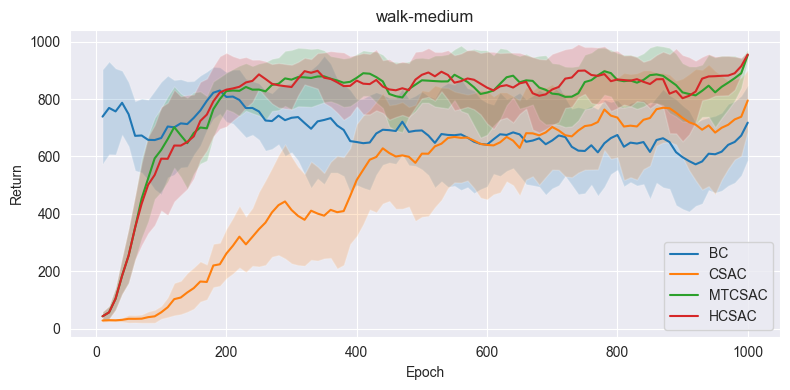
\includegraphics[width=0.45\textwidth]{figure/walk_medium.png}
    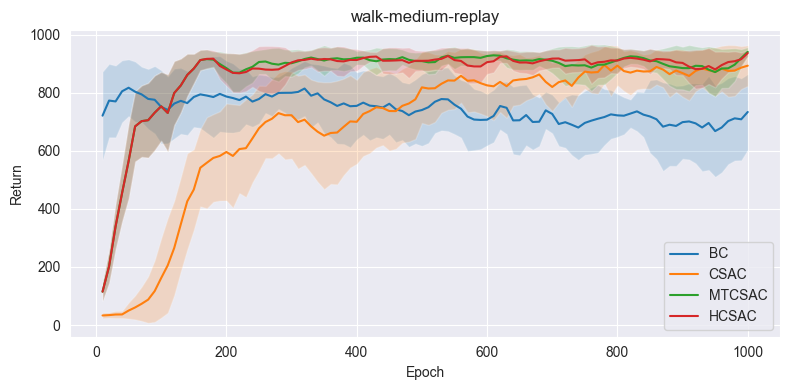
\includegraphics[width=0.45\textwidth]{figure/walk_medium_replay.png}
    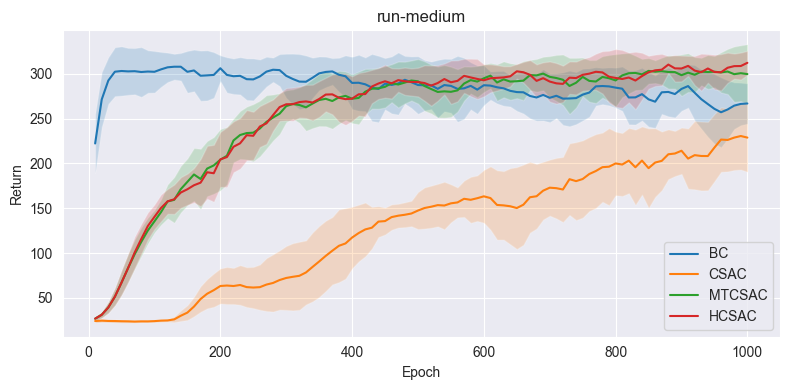
\includegraphics[width=0.45\textwidth]{figure/run_medium.png}
    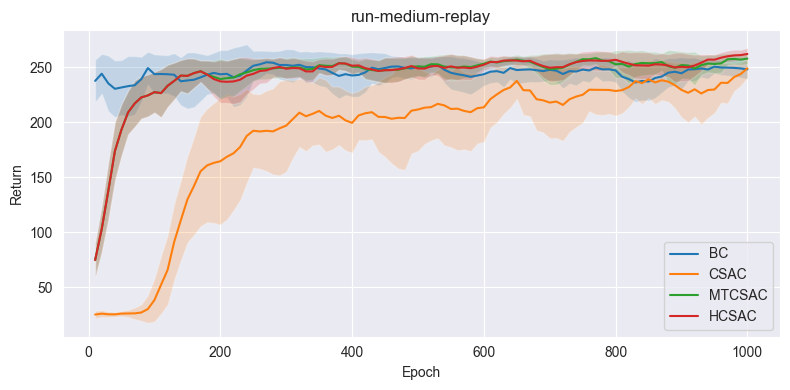
\includegraphics[width=0.45\textwidth]{figure/run_medium_replay.png}
    \caption{Training curves of the agents on the Walker2D environment. The top row shows the results of the \texttt{walk} task and the bottom row shows the results of the \texttt{run} task. The left column shows the results of the \texttt{medium} dataset and the right column shows the results of the \texttt{medium-replay} dataset.}
    \label{fig:experiment_result}
\end{figure}

Figure \ref{fig:experiment_result} shows the training curves of the agents on the Walker2D environment. We can see that MTCSAC (green curve) and HCSAC (red curve) significantly outperform CSAC (orange curve) in all the tasks, which demonstrates that the multi-task setting benefits the training process so that the agent can learn useful shared representations from different tasks. HCSAC performs slightly better than MTCSAC in majority of the training process, especially for the \texttt{medium} quality dataset, which indicates that the heuristic relabeling method can effectively augment the offline dataset so that the agent can learn from more valuable transitions. We can expect that HCSAC will achieve even better performance on the dataset with higher quality. The averages return in the \texttt{run} task are much lower than those in the \texttt{walk} task because the former is more challenging and requires precise control, which is consistent with the sampled trajectories in the offline dataset.

\begin{table}[ht]
    \caption{Performance evaluation of the agents on the Walker2D environment. The experiments are divided into two groups according to the dataset used for training, each containing two tasks. Every single experiment is conducted with $5$ different random seeds and the returns are reported in the form of mean and standard deviation. The best results are highlighted in bold.}
    \label{tab:performance_evaluation}
    \centering
    {\small \begin{tabular}{cccccc}
        \toprule
        \textbf{Dataset} & \textbf{Task} & \textbf{BC} & \textbf{CSAC} & \textbf{MTCSAC} & \textbf{HCSAC} \\
        \midrule
        \multirow{3}{*}{\texttt{medium}} & \texttt{walk} & $551.52 \pm 125.24$ & $653.57 \pm 233.83$ & $870.06 \pm 92.99$ & $\bm{907.38 \pm 67.39}$ \\
        & \texttt{run} & $\bm{317.26 \pm 9.46}$ & $213.67 \pm 49.56$ & $306.16 \pm 20.43$ & $308.38 \pm 7.64$ \\
        & \texttt{average} & $434.39 \pm 67.35$ & $433.62 \pm 141.70$ & $588.11 \pm 56.71$ & $\bm{607.88 \pm 37.52}$ \\
        \midrule
        \multirow{3}{*}{\texttt{replay}} & \texttt{walk} & $829.63 \pm 74.64$ & $812.80 \pm 146.82$ & $\bm{931.37 \pm 9.21}$ & $927.43 \pm 14.76$ \\
        & \texttt{run} & $244.80 \pm 33.35$ & $234.81 \pm 22.11$ & $254.31 \pm 11.60$ & $\bm{256.79 \pm 10.13}$ \\
        & \texttt{average} & $537.22 \pm 53.00$ & $523.81 \pm 84.47$ & $\bm{592.84 \pm 10.41}$ & $592.11 \pm 12.44$ \\
        \bottomrule
    \end{tabular}}
\end{table}

Table \ref{tab:performance_evaluation} shows the quantitative evaluation of the agents on the Walker2D environment. We provide behavioral cloning (BC) as the weak baseline. CSAC is selected as the strong baseline without multi-task learning. According to the given quantitative results, MTCSAC and HCSAC achieve higher average returns with lower standard deviations compared to CSAC in most settings, which indicates that our proposed multi-task learning methods including task embedding and heuristic relabeling in general bring superior performance and improve the robustness of the agent.
\section{Conclusion}
\label{sec:conclusion}

In this project, we propose a novel method named heuristic conservative soft actor-critic (HCSAC) to solve the offline multi-task reinforcement learning problem. The method is developed based on the classic algorithms of conservative Q-learning (CQL) and soft actor-critic (SAC) to suppress distribution shifts in the offline setting. We further propose task embedding to allow the agent to learn shared representations across multiple tasks. In addition, we follow conservative data sharing (CDS) to propose heuristic relabeling to augment the offline dataset, so that the agent can benefit from the shared transitions while avoiding performance degradation. We conduct a series of experiments on the MuJoCo benchmark to verify the effectiveness of our method. The results show that our proposed methods in general bring superior performance and improve the robustness of the agent.

We should point out that it is not sufficient to evaluate our methods only on the MuJoCo benchmark. On one hand, the offline transitions are only shared across two tasks, where \texttt{walk} and \texttt{run} are both low-level locomotion skills, so it is unnecessary to share any part of the policy. In real-world scenarios, we actually expect the agent can learn from a large number of tasks to acquire those essential skills. On the other hand, MuJoCo is an environment with low-dimensional state spaces where the vectorized observations already contain all the information needed for robotic control, so the multi-task learning methods cannot be fully exploited. We assert that our methods will show more advantages in the high-dimensional vision-based environments, where the agent can utilize transitions from different tasks to learn better shared representations.

\bibliographystyle{plain}
\bibliography{references}

\appendix

\section{Member Contribution}
\label{app:member_contribution}

All the members contribute equally to this project, and the specific contributions are as follows:

\noindent \textbf{Jiazi Bu.} Investigate the related work about the provided topic, participate in the discussion of the framework design, and complete part of the report writing.

\noindent \textbf{Kailing Wang.} Run the experiments including model training and evaluation, analyze the results, tune the hyperparameters, and complete part of the report writing.

\noindent \textbf{Xiangyuan Xue.} Participate in the discussion of the framework design, implement the code of the proposed method, complete part of the report writing, and finally present the project.

\end{document}